\chapter{Summary}


This document helps to understand issues related to determinism and robustness
in a White Rabbit Network. The final system's performance is a result of
connecting a number of existing technologies/techniques/standards, extending
them and providing hardware support. These are depicted in
Figure~\ref{fig:osiLayers} with reference to the OSI Model. 


\begin{center}
	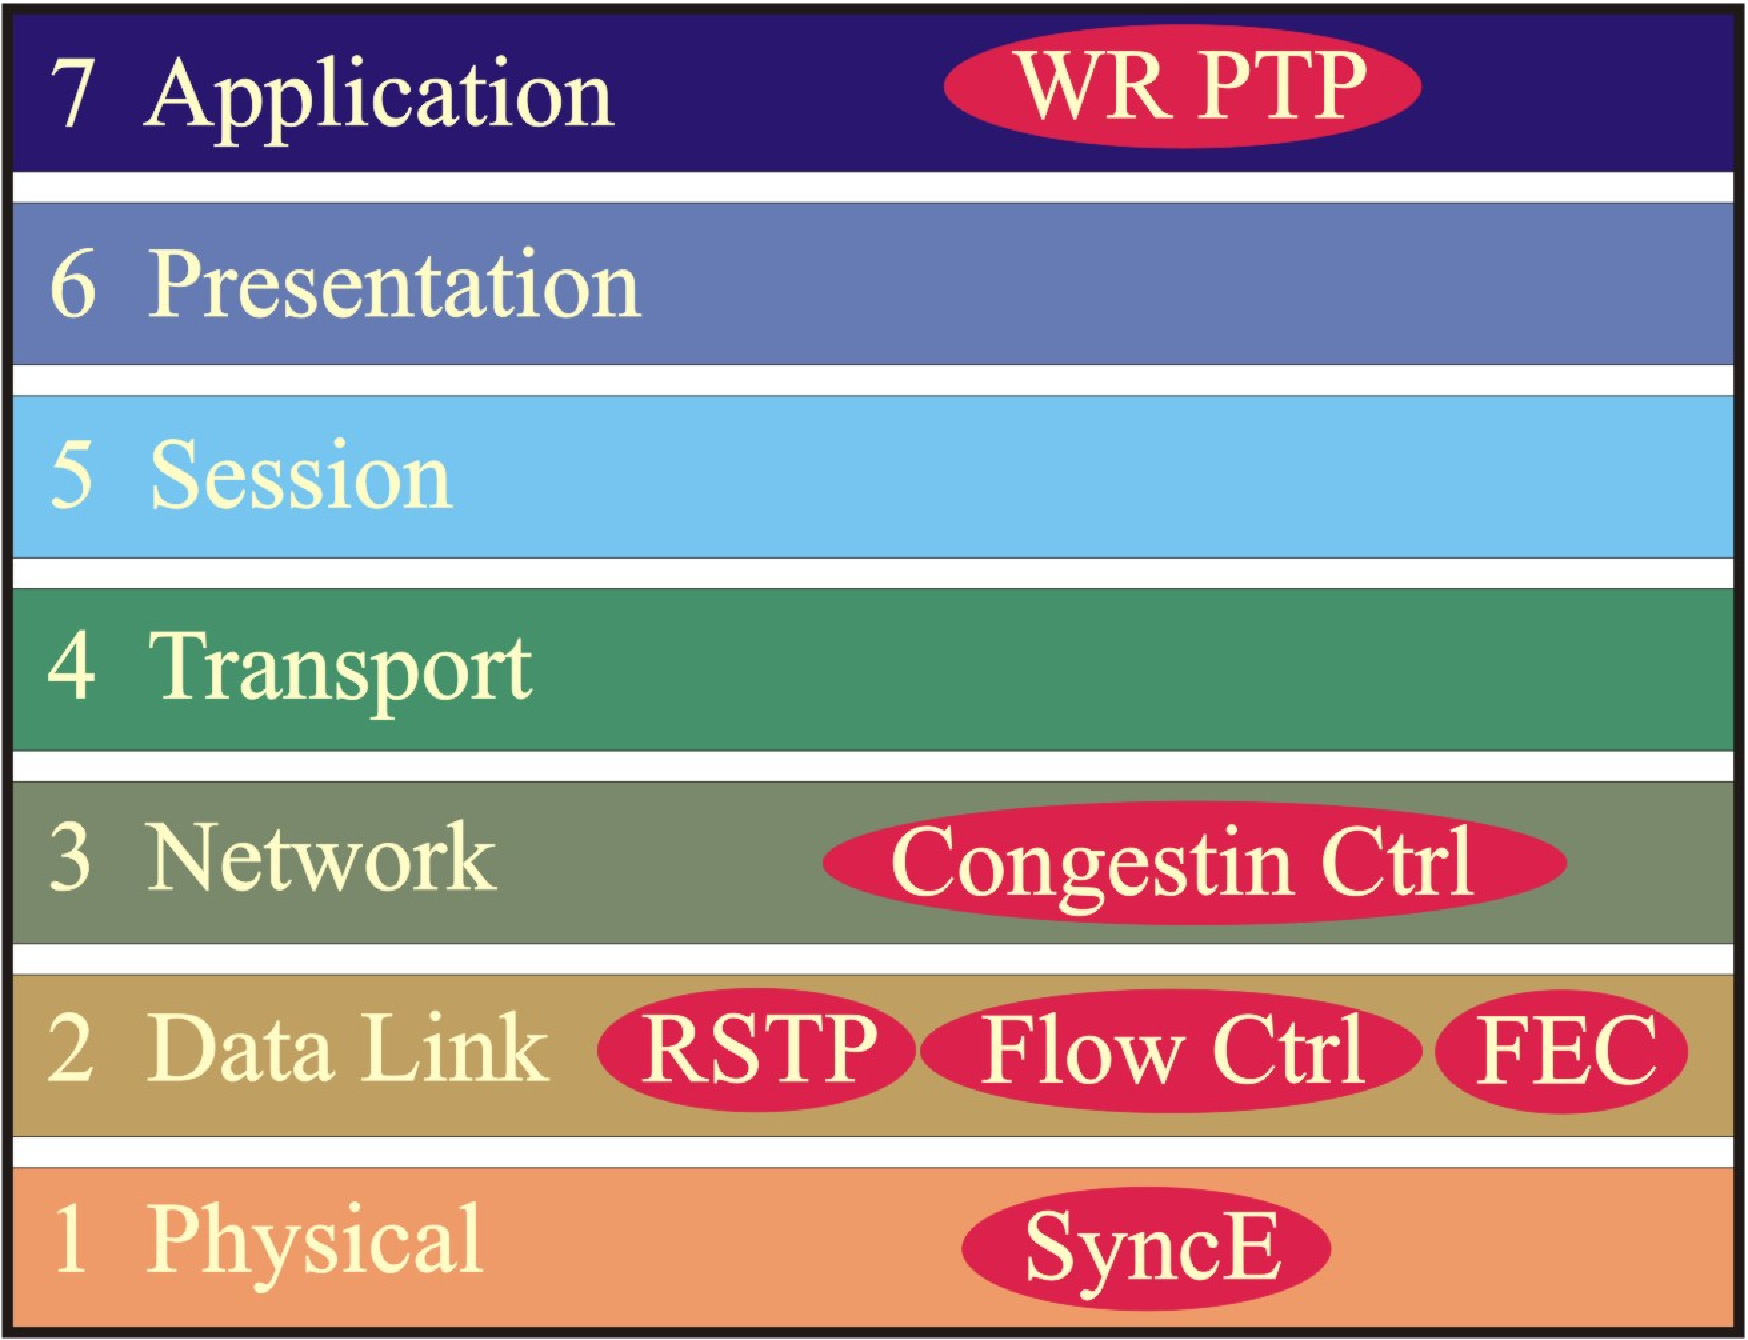
\includegraphics[scale=0.35]{robustness/osiLayers.png}
	\captionof{figure}{Placing methods used in WR according to OSI Layers.}
	\label{fig:osiLayers}
\end{center}

The topics which this document shall bring under discussion are:
\begin{itemize}
    \item We might need to consider dropping frames when \HP\ Package arrives in
order to decrease \ControlMessage\ jitter. Influence of such solution
on \SP\ Traffic's throughput needs to be tested.
    \item GSI's requirement of 100$\mu s$ should be more thoroughly justified as
it requires extensive efforts to achieve (e.g. \HP\ Bypass).
    \item The estimations of reliability presented in
Chapter~\ref{WRnetworkTopologyExamples} indicates that it is required to
provide triple or higher redundancy of the network in order to meet the
reliability requirement. Therefore:
   \begin{itemize}
      \item the implementation of $N > 2$ uplink ports in V3 Switch is desired,
      \item thorough calculations of reliability for various topologies need to
	    be conducted this.
   \end{itemize}
 \item Calculation of the overall WR Network
reliability turned out to be
much harder then anticipated. The current estimations need to be verified and
more precise calculations provided in further versions of the document.
\end{itemize}



